% vim: set tw=78 tabstop=4 shiftwidth=4 aw ai:
\documentclass{beamer}

\usepackage[utf8x]{inputenc}		% diacritice
\usepackage[english]{babel}
\usepackage{color}			% highlight
\usepackage{alltt}			% highlight
\usepackage{multicol}
\usepackage{underscore}

% highlight; comment this out in case you don't input code source files
% \usepackage{code/highlight}		% highlight

\usepackage{hyperref}			% folosiți \url{http://...}
					% sau \href{http://...}{Nume Link}
\usepackage{verbatim}
\usepackage{wasysym}
\usepackage{subfigure}

% Show contents at every section beginning. Ripped off from manual.
\AtBeginSection[] % Do nothing for \section*
{
	\begin{frame}<beamer>
		\frametitle{Outline}
	\tableofcontents[currentsection]
		\end{frame}
}

\mode<presentation>
{ \usetheme{Pittsburgh} \usecolortheme{seahorse} }

\setbeamertemplate{footline}[institute]{}

% Încărcăm simbolurilor Unicode românești în titlu și primele pagini
\PreloadUnicodePage{200}

\author{
		{\hspace{3mm} Adriana Costin \hspace{12mm}  Adrian Stanciu}
		\newline
		{Mihai Maruseac \hspace {10mm} Irina Grădinaru \hspace{10mm}
		Adrian Șendroiu}}
\title{Advances in Information Retrieval}

\institute[ACS UPB]{Faculty of Automatic Control and Computer Science \\
					Politehnica University of Bucharest}
\date{January 11, 2013}

\begin{document}

% Slide-urile cu mai multe părți sunt marcate cu textul (cont.)
\setbeamertemplate{frametitle continuation}[from second]

% Arătăm numărul frame-ului
% \setbeamertemplate{footline}[frame number]

\frame{\titlepage}

\frame{\tableofcontents}

% NB: Secțiunile nu sunt marcate vizual, ci doar apar în cuprins
\section{Dummy}

\begin{frame}{Cattitude}
	\begin{columns}
		\begin{column}[l]{0.2\textwidth}
		\begin{itemize}
			\item miau1
			\item miau2
			\item miau3
		\end{itemize}

		\end{column}
		\begin{column}[l]{0.8\textwidth}
			\begin{figure}
				
\includegraphics[scale=1.5]{img/cat.jpg}
			\end{figure}
		\end{column}
	\end{columns}
\end{frame}


\subsection{Query Recommendation}

% următoarele 2 slide-uri merg aici pe post de introducere? sau separat?

\begin{frame}{Human Perception of Query Quality}

\begin{quote}
How do users rate the quality of a query?
\end{quote}

\vspace{10pt}

Judging by search problem / query features:
	\begin{itemize}
		\item high specificity
		\item longer queries (4-5 words)
		\item comparing to what query they would personally use
		\item queries for fact-finding problems rated lower than\\ queries for
		exploratory problems % formulare prea verbose
		\begin{itemize}
			\item fact-finding: height of the Eiffel Tower
			\item exploratory: wildlife in the Masoala National Park
		\end{itemize}
	\end{itemize}
After viewing a results page:
	\begin{itemize}
		\item number of relevant results out of those viewed % pe grafic
		\item result rank is not as good an indicator
	\end{itemize}

\end{frame}

\begin{frame}{Query Quality vs Result Relevance}
\begin{figure}
	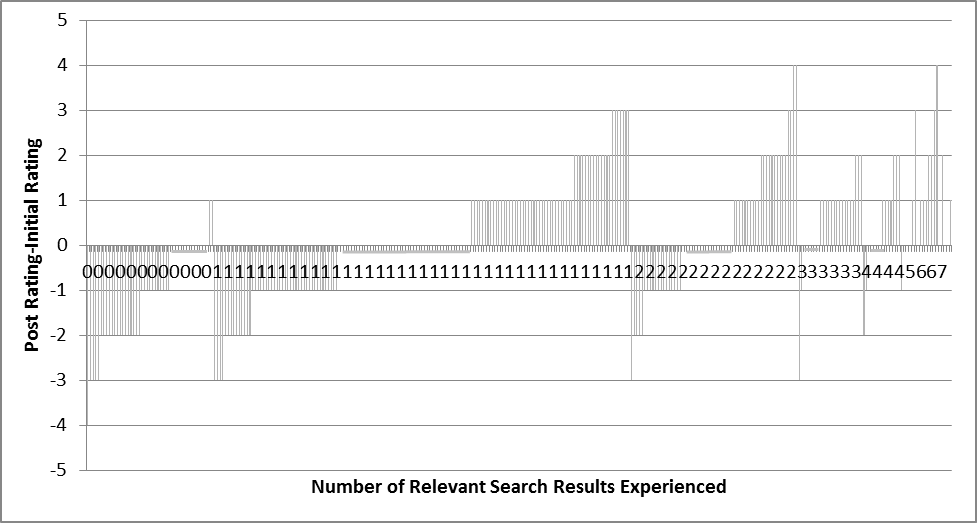
\includegraphics[width=0.8\textwidth]{img/qquality.png}
\end{figure}
Difference in query rating \textbf{before} and \textbf{after} viewing the result page
\begin{itemize}
	\item 0 relevant results clicked: lower rating
	\item 1-2 relevant results clicked: undetermined
	\item 3 or more relevant results clicked: higher rating
\end{itemize}
\end{frame}

\begin{frame}{Query Recommendation}

Suitable refinements to an initial query

\end{frame}


\begin{frame}{Query Recommendation on Intranets}

Document collection on Intranet:
\begin{itemize}
	\item relatively small
	\item changes less frequently (than Internet)
	\item more limited context of search (than Internet) \newline
\end{itemize}

Methods for Query Recommendation on Intranets:
\begin{itemize}
	\item concept hierarchy
	\item search logs
\end{itemize} 

\end{frame}


\begin{frame}{The Concept Hierarchy Model (CHM)}

What is a concept?
\begin{itemize}
	\item keyword
	\item phrase
	\item n-grams \newline
\end{itemize}

Concept Hierarchy:
\begin{itemize}
	\item created from a document collection
	\item used for ranking terms according to the strength of their links to the query within the hierarchy
\end{itemize}

\end{frame}


\begin{frame}{Subsumption Hierarchy for REsult Clustering (SHReC)}

Use term co-occurence to build a subsumption hierarchy tree \newline

For each concept (node in graph):
\begin{itemize}
	\item all direct ascendants are generalizations for the current concept
	\item all direct descendants are specializations for the current concept \newline
\end{itemize}

Static hierarchy with a high computational cost to frequently rebuild it 

\end{frame}


\begin{frame}{Query Recommendation using Search Logs}

Types:
\begin{itemize}
	\item local (based only on each user's previous searches)
	\item global (based on all previous searches) \newline
\end{itemize}

Query Flow Graph
\begin{itemize}
	\item state-of-the-art log-based query recommender
	\item directed graph:
		\begin{itemize}
			\item nodes contain queries
			\item edges represent query refinements \newline
		\end{itemize}
\end{itemize}

Dynamic structure and easy to be updated

\end{frame}


\begin{frame}{Adaptation of CHM with Search Logs}

Concept Hierarchy discovers relationships between terms based on statistical analysis, giving a conceptual view \newline

Search Logs provide a conceptual view based on collective user intelligence \newline

Two complementary conceptual views on the same search domain
$ \Rightarrow $
Adapt the CHM with user interactions derived from Search Logs

\end{frame}


\begin{frame}{SHReC Results}

Adaptive SHReC is more efficient than QFG, which is more efficient that static SHReC \newline

Users will benefit more from the models when all log refinements are used for adaptation rather than only those with clicks

\end{frame}



\subsection{Context-Aware Ranking}


\begin{frame}{Context-Aware Ranking}

Main problems:
\begin{itemize}
	\item how can we take advantage of different types of contexts in ranking?
	\item how can we integrate context information into a ranking model? \newline
\end{itemize}

Context contains:
\begin{itemize}
	\item queries asked before the current query in the same session
	\item answers to those queries (clicked or skipped by the user) \newline
\end{itemize}

\end{frame}


\begin{frame}{Context-Aware Ranking Principles}

Relations between queries in the same session:
\begin{itemize}
	\item unrelated
	\item reformulation
	\item specialization
	\item generalization
	\item general association
\end{itemize}

\end{frame}


\begin{frame}{Reformulation}

Example: \newline
'homes for rent in atlanta' $ \rightarrow $ 'houses for rent in atlanta' \newline

Why? \newline
- search results of the previous query do not or only partially fulfill the information need \newline

Principle:
\begin{quotation}
for consecutive queries $ q_{t-1}q_{t} $ in a session such that $ q_{t} $ reformulates $ q_{t-1} $, if a search result \emph{r} for $ q_{t-1} $ is clicked on or skipped, \emph{r} as a result for $ q_{t} $ is unlikely to be clicked on and thus should be demoted
\end{quotation}

\end{frame}


\begin{frame}{Specialization}

Example: \newline
'time life music' $ \rightarrow $ 'time life Christian CD' \newline

Why? \newline
- see more specific results \newline

Principle:
\begin{quotation}
for consecutive queries $ q_{t-1}q_{t} $ in a session such that $ q_{t} $ specializes $ q_{t-1} $, the user likely prefers the search results specifically focusing on $ q_{t} $
\end{quotation}

Implementation: \newline
- promote the results matching $ q_{t} \setminus q_{t-1} $ in the set of answers to $ q_{t} $

\end{frame}


\begin{frame}{Generalization}

Example: \newline
'free online Tetris' $ \rightarrow $ 'Tetris game' \newline

Why? \newline
- get information not covered by the previous query \newline

Principle:
\begin{quotation}
for consecutive queries $ q_{t-1}q_{t} $ in a session such that $ q_{t} $ generalizes $ q_{t-1} $, the user would likely not prefer the search results specifically focusing on $ q_{t-1} $
\end{quotation}

Implementation: \newline
- demote the results matching $ q_{t-1} \setminus q_{t} $ in the set of answers to $ q_{t} $

\end{frame}


\begin{frame}{General Association}
\begin{small}

Example: \newline
'Xbox 360' $ \rightarrow $ 'FIFA 2010' \newline

Why? \newline
- when an ambiguous query is generally associated with its context, the context may help to narrow down the user's search intent \newline

Principle:
\begin{quotation}
for consecutive queries $ q_{t-1}q_{t} $ in a session such that $ q_{t} $ and $ q_{t-1} $ are generally associated, the user likely prefers the search results related to both $ q_{t-1} $ and $ q_{t} $
\end{quotation}

Implementation:
\begin{itemize}
	\item choose a topic taxonomy (such as Open Directory Project: http://www.dmoz.org)
	\item let $ C_{t-1} $ and $ C_{t} $ be the sets of topics of $ q_{t-1} $ and $ q_{t} $, and $ C_{\cap} $ the set of common topics between $ C_{t-1} $ and $ C_{t} $; promote a search result \emph{r} if the set of topics of \emph{r} shares at least one topic with $ C_{\cap} $
\end{itemize}

\end{small}
\end{frame}


\begin{frame}{Learning to rank}

Supervized machine learning problem in which the goal is to automatically construct a ranking model from training data \newline

RankSVM – learn a SVM model for classification on the preference between a pair of documents \newline

Derive features from the ranking principles and incorporate them into the RankSVM model

\end{frame}



\subsection{Web Spam Detection}

\begin{frame}{Web Spam}

What constitutes web spam?

\begin{itemize}

\item auto-generated web pages that contain:

\begin{itemize}
	\item common search keywords and phrases
	\item "borrowed" content from many different pages
	\item advertisements
\end{itemize}

\item produce ad revenue by attracting traffic

\item little or no informative value to the user

\end{itemize}

What we want - detect and eliminate web spam from search results
\end{frame}

\begin{frame}{Quilted Pages}

"Quilted" page:
\begin{itemize}
	\item page made up of content borrowed from other web pages
	\item content usually comes from other domains
\end{itemize}

\begin{quote}
	Warning! Not all quilted pages are web spam.
	% blog front pages, news portals, lyrics sites, ...
\end{quote}

Using an algorithm that detects \textbf{all} quilted pages:
\begin{itemize}

\item quilt parameters:
\begin{itemize}
	\item number of sources for the content
	\item size of shingles taken into account
	\item eliminating common shingles
\end{itemize}

\item final result: only 34\% of the quilted pages were spam 
% your algorithm is bad, and you should feel bad

\item possible improvements:
\begin{itemize}
	\item semantic analysis of page content
	\item recognition by other features of web spam pages
\end{itemize}

\end{itemize}

\end{frame}

\begin{frame}{Spam Analysis}
Prevalent features of web spam:
\begin{itemize}
	\item large number of words per page - keyword stuffing
	\item long words - "freedownloads", "hotelbookings"
	\item lots of \textbf{anchor words}
	\item many words in title - for SEO % grafic 1
	\item high compression ratio - redundancy due to repeated words % grafic 2
	\item high proportion of visible content - less markup  % grafic 3
	\item small number of stop words % grafic 4
	% sunt clare astea? ar mai merge explicitate
\end{itemize}
\end{frame}

\begin{frame}[plain]
\begin{figure}
\centering

% 	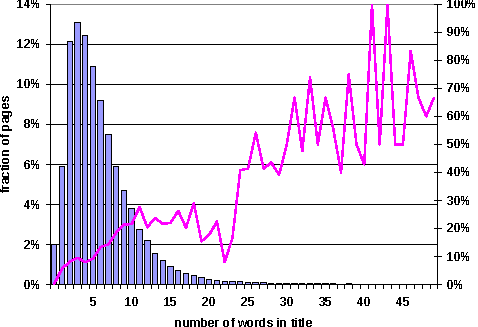
\includegraphics[width=0.5\textwidth]{img/webspam-title.pdf}
% 	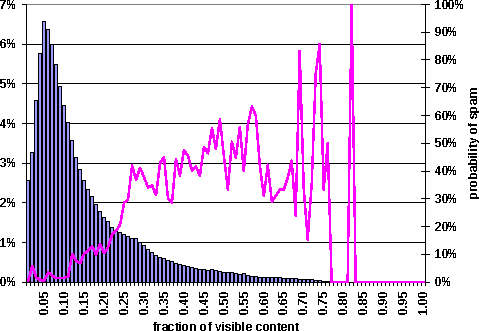
\includegraphics[width=0.5\textwidth]{img/webspam-visible.pdf}
%	\newline
% 	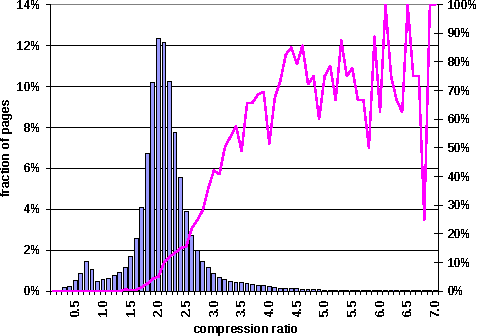
\includegraphics[width=0.5\textwidth]{img/webspam-compression.pdf}
% 	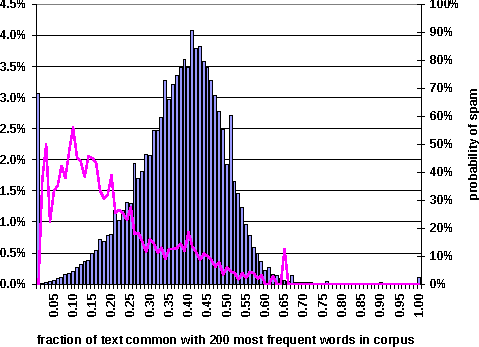
\includegraphics[width=0.5\textwidth]{img/webspam-stopwords.pdf}

 	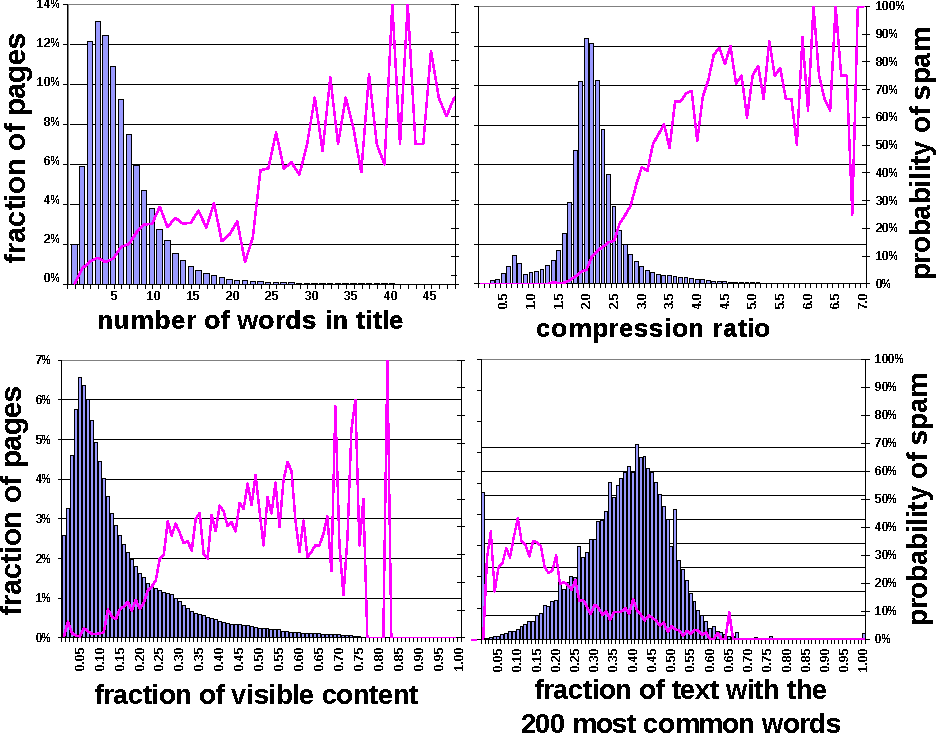
\includegraphics[width=\textwidth]{img/webspam-all.pdf}
\end{figure}
\end{frame}

\begin{frame}{Spam Detection}
\begin{columns}
	\begin{column}[r]{0.6\textwidth}
	How do we use these features?
	\begin{itemize}
	\item compute numeric ranges for each feature
	\item build a \textbf{decision tree}-based classifier
	\end{itemize}
	\end{column}

	\begin{column}[l]{0.5\textwidth}
		\begin{figure}
		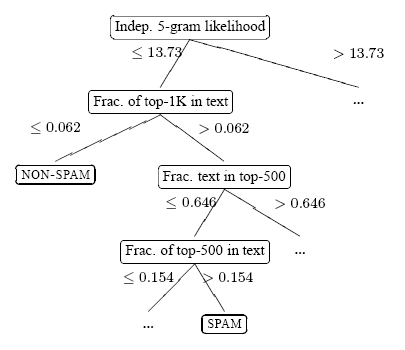
\includegraphics[width=\textwidth]{img/dtree.png}
		\end{figure}
	\end{column}
\end{columns}

Results:
\begin{itemize}
	\item spam: 91.1\% precision, 86.2\% recall
	\item non-spam: 98.7\% precision, 97.8\% recall
\end{itemize}
\end{frame}


\section{Trends and Ideas}

\begin{frame}{Trends and Ideas}

Ce-a zis profu în mail:
\begin{quotation}
	 Puneti la final o sectiune cu:
	\begin{itemize}
		\item Trenduri (ce vi se pare voua ca e la moda pe directia aia acum).
		\item Idei (ce credeti ca s-ar putea face pentru a avansa directia respectiva).
	\end{itemize}
	
\end{quotation}

\end{frame}


\end{document}
